%File: sokrates.tex
\documentclass[letterpaper]{article} % DO NOT CHANGE THIS
\usepackage{aaai2026}  % Camera-ready (single-blind workshop)
\usepackage{times}  % DO NOT CHANGE THIS
\usepackage{helvet}  % DO NOT CHANGE THIS
\usepackage{courier}  % DO NOT CHANGE THIS
\usepackage[hyphens]{url}  % DO NOT CHANGE THIS
\usepackage{graphicx} % DO NOT CHANGE THIS
\urlstyle{rm} % DO NOT CHANGE THIS
\def\UrlFont{\rm}  % DO NOT CHANGE THIS
\usepackage{natbib}  % DO NOT CHANGE THIS AND DO NOT ADD ANY OPTIONS TO IT
\usepackage{caption} % DO NOT CHANGE THIS AND DO NOT ADD ANY OPTIONS TO IT
\frenchspacing  % DO NOT CHANGE THIS
\setlength{\pdfpagewidth}{8.5in} % DO NOT CHANGE THIS
\setlength{\pdfpageheight}{11in} % DO NOT CHANGE THIS
%
% Math packages (allowed for mathematics)
\usepackage{amsmath}
\usepackage{amssymb}
%
% TikZ for diagrams
\usepackage{tikz}
\usetikzlibrary{shapes, arrows.meta, positioning, calc, fit, backgrounds, shadows}
%
% These are recommended to typeset algorithms but not required.
\usepackage{algorithm}
\usepackage{algorithmic}
%
% These are recommended to typeset listings but not required.
\usepackage{newfloat}
\usepackage{listings}
\DeclareCaptionStyle{ruled}{labelfont=normalfont,labelsep=colon,strut=off} % DO NOT CHANGE THIS
\lstset{%
	basicstyle={\footnotesize\ttfamily},% footnotesize acceptable for monospace
	numbers=left,numberstyle=\footnotesize,xleftmargin=2em,% show line numbers
	aboveskip=0pt,belowskip=0pt,%
	showstringspaces=false,tabsize=2,breaklines=true}
\floatstyle{ruled}
\newfloat{listing}{tb}{lst}{}
\floatname{listing}{Listing}
%
\pdfinfo{
/TemplateVersion (2026.1)
}

\setcounter{secnumdepth}{0} %May be changed to 1 or 2 if section numbers are desired.

% Custom commands for this paper
\newcommand{\qhat}{\hat{q}_\phi}
\newcommand{\sokrates}{Sokrates}
\newcommand{\oak}{OaK}
\newcommand{\dpo}{DPO}

\title{SOKRATES: Distilling Symbolic Knowledge into Option-Level Reasoning via Solver-Guided Preference Optimization}
\author{
    Zhaoxiang Feng\textsuperscript{\rm 1},
    David Scott Lewis\textsuperscript{\rm 2}
}
\affiliations{
    \textsuperscript{\rm 1}University of California San Diego, USA\\
    \textsuperscript{\rm 2}AI Executive Consulting (AIXC), Zaragoza, Spain\\
    zhf004@ucsd.edu, reports@aiexecutiveconsulting.com
}

\begin{document}

\maketitle

\begin{abstract}
A language model that achieves $94\%$ accuracy on logical reasoning sounds impressive---until you discover that only $2\%$ of its proofs are actually valid. This is the state of chain-of-thought prompting: models produce plausible rationales that frequently contain invalid inference steps, hidden contradictions, or skipped derivations. The right answer emerges \emph{despite}, not \emph{because of}, the reasoning process. We introduce \sokrates{} (\textbf{S}ymbolic \textbf{O}ption-\textbf{K}nowledge \textbf{R}easoning \textbf{A}lignment via \textbf{T}race \textbf{E}valuation with \textbf{S}olver), a method that instantiates Sutton's Options and Knowledge (\oak{}) framework in a first-order logic micro-world. \sokrates{} represents proofs as sequences of discrete inference-rule \emph{options} (e.g., \texttt{MODUS\_PONENS}, \texttt{UNIV\_INST}), verified step-by-step by a FOL solver. From solver feedback we (i)~train an option-success predictor $\qhat(s,\omega)$ that estimates validity before execution, and (ii)~construct preference pairs for Direct Preference Optimization (\dpo{}), aligning the model's option policy with solver-induced correctness. On PrOntoQA, \sokrates{} raises accuracy from $94.2\%$ to $97.6\%$, step validity from $27.3\%$ to $98.5\%$, and full-trace validity from $2.1\%$ to $92.0\%$---a \textbf{33$\times$ improvement} in logically sound proofs. The learned $\qhat$ is well calibrated (ECE~$= 0.08$), and the option policy transfers zero-shot to FOLIO, improving accuracy from $45.3\%$ to $53.2\%$. To our knowledge, \sokrates{} is the first closed-loop \oak{} instantiation in a neural language model, demonstrating that the options-and-knowledge paradigm yields substantial empirical gains in symbolic reasoning.
\end{abstract}

%============================================================================
\section{Introduction}
%============================================================================

Large language models have shown impressive multi-step reasoning capabilities when prompted with chain-of-thought (CoT) explanations \cite{wei2022chain} and sampled with self-consistency decoding \cite{wang2023selfconsistency}.
However, closer inspection reveals a troubling pattern: their intermediate reasoning is frequently wrong even when the final answer is correct.
Proofs contain logically invalid steps, missing premises, or contradictions that a symbolic checker would reject \cite{saparov2023language, huang2024large}.
This ``right answer, wrong reasoning'' phenomenon makes such systems difficult to trust in domains where intermediate steps must be sound.

Two families of neuro-symbolic methods attempt to close this gap.
Semantic loss approaches such as LoCo-LMs and Logical Neural Networks \cite{riegel2020logical} incorporate differentiable logical constraints into the training objective, encouraging local consistency of token-level predictions but leaving the global proof process implicit.
Solver-augmented CoT approaches such as Logic-LM \cite{pan2023logic} and LINC \cite{olausson2023linc} parse CoTs into first-order logic (FOL) and invoke external theorem provers to verify or repair them.
These methods improve faithfulness, but they still treat reasoning as unstructured text and do not learn explicit predictive models of which reasoning \emph{actions} will succeed in which states.

We argue that logical reasoning is more naturally viewed as a sequential decision problem over \emph{inference rules}: at each step, the agent must decide which rule to apply and to which premises.
This perspective aligns with Sutton's Options and Knowledge (\oak{}) framework \cite{sutton2023reward}, which advocates that agents should learn (1) a reusable vocabulary of temporally extended behaviors (\emph{options}) and (2) explicit predictive models of how those options behave (\emph{knowledge}).
In a logic micro-world, inference rules such as Modus Ponens or Universal Instantiation are precisely such options, and a FOL solver can act as a source of ground-truth knowledge about their success.

We introduce \sokrates{}, a system that instantiates this program for LLM-based logical reasoning.
Proofs are represented as sequences of discrete options drawn from a small inference-rule vocabulary (Table~\ref{tab:options}).
A FOL solver checks each option application and returns either a validated derived formula or an error.
From this signal we learn two coupled components:
(i) an option-success predictor $\qhat(s,\omega)$ that estimates the probability that option $\omega$ will be solver-valid in state $s$; and
(ii) an option policy updated via solver-guided \dpo{}, which builds preferences between better and worse traces based on step-level validity and final correctness.
Figure~\ref{fig:architecture} summarizes this micro \oak{} loop.

Concretely, we make the following contributions:
\begin{itemize}
    \item \textbf{Optionized reasoning.} We cast proof construction as control over a finite option set of inference-rule macros with structured arguments, and generate reasoning traces in a Thought/Action format inspired by ReAct \cite{yao2023react}.
    
    \item \textbf{Explicit option knowledge.} We train an option-success head $\qhat(s,\omega)$ on solver labels, providing a calibrated, per-step estimate of logical validity for each option in context.
    
    \item \textbf{Solver-guided preference optimization.} We construct solver-derived preferences over optionized traces and apply \dpo{} \cite{rafailov2023direct} to align the option policy with stepwise logical correctness, yielding a concrete \oak{} loop for symbolic reasoning with LLMs.
\end{itemize}

On PrOntoQA, \sokrates{} substantially improves both task performance and reasoning soundness: relative to an optionized supervised fine-tuning (SFT) baseline, accuracy rises from $94.2\%$ to $97.6\%$, while step validity jumps from $27.3\%$ to $98.5\%$ and the fraction of fully valid traces from $2.1\%$ to $92.0\%$ (Table~\ref{tab:main_results}).
The learned option policies also transfer zero-shot to FOLIO, and the option head $\qhat$ is well calibrated under Brier score and ECE, indicating that the model has acquired nontrivial predictive knowledge about its own reasoning steps.
To our knowledge, \sokrates{} represents the first closed-loop instantiation of the \oak{} framework in a neural language model.

% Architecture figure (moved to Introduction per improvement suggestions)
% Old version preserved in figures/architecture.tex
% Architecture diagram v2 - Updated layout with improved visual design
% Note: This file is for inclusion in the main paper, not standalone compilation
% For standalone compilation, see architecture_v2_standalone.tex

% --- Colors ---
\definecolor{myblue}{RGB}{218, 232, 252}   % Data/Blue
\definecolor{mygreen}{RGB}{213, 232, 212}  % Init/Green
\definecolor{myorange}{RGB}{255, 224, 204} % Loop/Orange
\definecolor{mypurple}{RGB}{225, 213, 231} % Solver/Purple
\definecolor{myred}{RGB}{248, 206, 204}    % Output/Red
\definecolor{mygrey}{RGB}{250, 250, 250}   % Background

% --- Macros (qhat defined in main document) ---
\newcommand{\pihat}{\pi^*}

\begin{figure*}[t]
\centering
\begin{tikzpicture}[
    scale=0.68, transform shape,
    node distance=1.2cm and 1.5cm,
    % Style Definitions
    base/.style={
        draw=black!60, 
        thick, 
        rounded corners=2pt, 
        align=center, 
        font=\small\sffamily,
        drop shadow={opacity=0.15},
        inner sep=6pt
    },
    data/.style={base, fill=myblue, minimum width=2.2cm, minimum height=1cm},
    process/.style={base, fill=myorange, minimum width=2.4cm, minimum height=1.1cm},
    model/.style={base, fill=mygreen, minimum width=2.2cm, minimum height=1cm},
    output/.style={base, fill=myred, minimum width=2.2cm, minimum height=1cm},
    solver/.style={base, fill=mypurple, minimum width=2.5cm, minimum height=1cm},
    arrow/.style={-Latex, thick, color=black!70},
    line/.style={thick, color=black!70}, % No arrow head
    dashed_arrow/.style={-Latex, thick, dashed, color=black!70},
    group_label/.style={font=\bfseries\itshape\color{black!60}, anchor=south} 
]
    % --- 1. Initialization Block ---
    \node[model] (sft) {SFT};
    \node[model, above=1.5cm of sft] (pi0) {$\pi_0$}; 

    % --- 2. Optionizer ---
    \node[process, left=2.0cm of $(sft.west)!0.5!(pi0.west)$] (optionizer) {Optionizer};

    % --- 3. Data Input ---
    \coordinate (data_x) at ($(optionizer.west) - (2.0cm, 0)$);
    \node[data] (pronto) at (data_x |- pi0) {PrOntoQA};
    \node[data] (folio) at (data_x |- sft) {FOLIO};

    % --- 4. Micro OaK Loop - Top Row ---
    \node[process, right=2.0cm of pi0] (gen) {Generate\\Traces};
    \node[process, right=1.0cm of gen] (verify) {Solver\\Verify};
    \node[process, right=1.0cm of verify] (update) {Update\\$\qhat$};

    % --- 5. Micro OaK Loop - Bottom Row ---
    \node[process] (build) at (verify |- sft) {Build\\Preferences};
    \node[process] (dpo) at (update |- sft) {DPO};

    % --- 6. Solver ---
    \node[solver, below=1.6cm of build] (z3) {Symbolic Solver};

    % --- 7. Outputs ---
    \node[output, right=2.0cm of update] (out_q) {Calibrated $\qhat^*$};
    \node[output] (out_pi) at (out_q |- dpo) {Aligned $\pihat$};

    % --- 8. Group Labels ---
    \coordinate (label_y) at ($(pi0.north) + (0, 0.4cm)$);
    \node[group_label] at (pronto |- label_y) {Data};
    \node[group_label] at (pi0 |- label_y) {Init};
    \node[group_label] at (out_q |- label_y) {Output};

    % --- Background Box ---
    \begin{scope}[on background layer]
        \coordinate (loop_top) at ($(update.north) + (0, 0.9cm)$);
        \coordinate (loop_bottom) at ($(dpo.south) - (0, 0.9cm)$);
        
        \node[
            draw=black!40, 
            thick, 
            dashed, 
            fill=mygrey, 
            rounded corners=10pt, 
            fit=(gen) (update) (loop_top) (loop_bottom),
            inner sep=0.5cm,
            label={[anchor=south, yshift=0.2cm]north:\textbf{\textit{Micro OaK Loop} (repeat $N$ iterations)}}
        ] (loop_box) {};
    \end{scope}

    % --- Connections ---
    % 1. Data -> Optionizer
    \coordinate (merge_point) at ($(pronto.east)!0.5!(optionizer.west)$);
    \draw[line] (pronto.east) -- (merge_point |- pronto.east);
    \draw[line] (folio.east) -- (merge_point |- folio.east);
    \draw[line] (merge_point |- pronto.east) -- (merge_point |- folio.east);
    \draw[arrow] (merge_point |- optionizer.west) -- (optionizer.west);

    % 2. Optionizer -> SFT
    \draw[arrow] (optionizer.south) |- (sft.west) node[pos=0.75, above, font=\scriptsize, align=center] {proof $\to$ \\ Thought/Action};
    
    % 3. SFT -> Pi0
    \draw[arrow] (sft.north) -- (pi0.south);

    % 4. Pi0 -> Generate
    \draw[arrow] (pi0.east) -- (gen.west);

    % 5. Loop Internal Flow
    \draw[arrow] (gen.east) -- (verify.west);
    \draw[arrow] (verify.east) -- (update.west);
    \draw[arrow] (verify.south) -- node[midway, right, font=\scriptsize] {Valid/Invalid} (build.north);
    \draw[arrow] (build.east) -- (dpo.west);

    % 6. Solver Connection
    \draw[arrow] (z3.north) -- (build.south);

    % 7. Output Connections
    \draw[arrow] (update.east) -- (out_q.west);
    \draw[arrow] (dpo.east) -- (out_pi.west);

    % --- Feedback Loops ---
    
    % DPO -> Generate (Bottom loop)
    \path (dpo.south) -- ++(0,-0.7) coordinate (bottom_bus);
    \draw[dashed_arrow, rounded corners] 
        (dpo.south) 
        -- (dpo.south |- bottom_bus) 
        -- node[pos=0.30, below, yshift=-2pt, font=\scriptsize] {Update Policy $\pi$} (gen.south |- bottom_bus) 
        -- (gen.south);

    % Update -> Generate (Top loop)
    \path (update.north) -- ++(0,0.7) coordinate (top_bus);
    \draw[dashed_arrow, rounded corners] 
        (update.north) 
        -- (update.north |- top_bus) 
        -- (gen.north |- top_bus) 
        -- (gen.north);

    % Text Annotations
    \node[font=\scriptsize, text=black!60, align=center] at ($(sft.south)+(0,-0.3)$) {format learning};

\end{tikzpicture}
\caption{The \sokrates{} architecture. We optionize proofs for SFT to obtain initial policy $\pi_0$, then repeat a micro \oak{} loop: generate traces, verify with a symbolic solver, update $\qhat$, build preferences, and apply \dpo{} to align the policy.}
\label{fig:architecture}
\end{figure*}



%============================================================================
\section{Background and Related Work}
%============================================================================

\subsection{LLM Reasoning and Failure Modes}

Chain-of-thought prompting \cite{wei2022chain} and self-consistency decoding \cite{wang2023selfconsistency} are the current workhorses for LLM reasoning, but they do not guarantee logically valid chains.
Systematic analyses reveal that LLMs are \emph{greedy reasoners}---locally good at individual deductions but poor at proof planning when many valid next steps exist \cite{saparov2023language}.
Furthermore, self-reflection without external feedback often fails to fix logical errors \cite{huang2024large}.

\sokrates{} tackles exactly this ``right answer, wrong reasoning'' regime by explicitly modeling which \emph{optionized} reasoning actions are solver-valid in which states, rather than relying on the surface plausibility of free-form thoughts.

\subsection{Logical Reasoning Benchmarks}

\paragraph{Synthetic Benchmarks.}
RuleTaker and ProofWriter \cite{clark2021transformers} provide synthetic rule-based reasoning with multi-hop proofs.
PrOntoQA \cite{saparov2023language} offers first-order synthetic worlds with formally analyzable CoT, making it ideal for isolating reasoning behavior.

\paragraph{Natural Language Benchmarks.}
FOLIO \cite{han2022folio} provides natural language premises with expert FOL annotations.
P-FOLIO extends it with human-written proof chains labeled with inference rules, which inform our option vocabulary.

We choose PrOntoQA as our primary testbed because it provides ground-truth proofs and fully specified FOL world models, enabling us to parse and verify every optionized step with a solver.

\subsection{Neuro-Symbolic Methods and Solver-Augmented Reasoning}

Prior work on integrating symbolic reasoning with LLMs falls into three categories:

\paragraph{LM + External Solver at Inference.}
LINC \cite{olausson2023linc} uses LLMs as semantic parsers to generate FOL, with external provers computing answers.
Logic-LM \cite{pan2023logic} parses CoT into FOL for solver verification and uses error messages for self-refinement.
LAMBADA \cite{kazemi2022lambada} employs backward-chaining control with LLM modules.
These approaches ``outsource'' proof search to symbolic engines but do not train an internal option model.

\paragraph{LMs Trained to Simulate Solvers.}
LoGiPT \cite{feng2024logipt} trains an LM on hidden intermediate steps of a deductive solver; the LM emulates the solver and can answer without external calls.
Unlike \sokrates{}, LoGiPT trains on full solver traces but does not decompose them into reusable option macros or learn a separate predictive head for step validity.

\paragraph{Neuro-Symbolic Consistency Objectives.}
LoCo-LMs and Logical Neural Networks \cite{riegel2020logical} incorporate differentiable logic constraints via semantic loss functions, encouraging consistency at the prediction level.
These operate on truth values or soft logical constraints, not on a structured sequence of options with explicit per-option success probabilities.

\paragraph{Positioning \sokrates{}.}
\sokrates{} is closest in spirit to Logic-LM and LoGiPT, in that it uses a symbolic solver to supervise reasoning, but differs by:
(i) factorizing reasoning into a finite option vocabulary,
(ii) learning an explicit option-success model $\qhat(s,\omega)$, and
(iii) using solver-derived preferences to shape an option policy via \dpo{} rather than directly imitating solver traces.

\subsection{Preference Learning and Process Supervision}

Direct Preference Optimization (\dpo{}) \cite{rafailov2023direct} provides an efficient alternative to PPO-style RLHF \cite{ouyang2022training} and has been widely adopted for LLM alignment.
Given preference pairs $(y_w, y_l)$ where $y_w$ is preferred over $y_l$, \dpo{} optimizes:
\begin{equation}
\mathcal{L}_{\text{DPO}} = -\mathbb{E}\left[\log \sigma\left(\beta \log \frac{\pi_\theta(y_w|x)}{\pi_{\text{ref}}(y_w|x)} - \beta \log \frac{\pi_\theta(y_l|x)}{\pi_{\text{ref}}(y_l|x)}\right)\right]
\label{eq:dpo}
\end{equation}
where $\pi_{\text{ref}}$ is a reference policy and $\beta$ controls the KL penalty.

\paragraph{Verifier-Based Preferences.}
VeriCoT \cite{ling2023deductive} translates CoT to FOL, verifies each step with a solver, and uses verification-based preferences for fine-tuning.
However, VeriCoT operates on \textbf{unstructured CoT text}, using a parser to extract predicates.
\sokrates{} instead uses a fixed \textbf{finite option set} with typed arguments (Table~\ref{tab:options}), trains an explicit knowledge head $\qhat(s,\omega)$ parallel to \dpo{}, and frames this as a micro \oak{} loop where option models are learned as predictive knowledge.

\subsection{Options, OaK, and Hierarchical RL}

The classic \textbf{options} framework \cite{sutton1999between} defines options as temporally extended actions with an initiation set, intra-option policy, and termination condition, enabling temporal abstraction and planning.

The \oak{} framework \cite{sutton2023reward} extends this by emphasizing that agents should learn not just policies but also \textbf{knowledge}---predictive models of how options behave.
\oak{} advocates \emph{reward-respecting subtasks} whose optimal policies do not conflict with the main objective.

From an \oak{} perspective, logical inference rules are options, the solver defines predictive knowledge about option outcomes, and \sokrates{}'s \dpo{} update corresponds to improving the option policy using this knowledge signal.
Importantly, our ``maintain logical consistency while answering the query'' subtask is reward-respecting: the main reward is correctness; the subtask reward is solver-validated step correctness; they are aligned, not competing.

%============================================================================
\section{Problem Setup: OaK in a Logic World}
%============================================================================

We cast logical reasoning as a sequential decision problem in a FOL micro-world where an agent incrementally constructs proofs by applying inference-rule options.
Table~\ref{tab:oak_mapping} makes explicit how \sokrates{} instantiates each component of the \oak{} framework.

% OaK mapping table
\begin{table}[t]
\centering
\caption{Mapping \sokrates{} to the Options and Knowledge framework.}
\label{tab:oak_mapping}
\footnotesize
\begin{tabular}{lp{2.8cm}p{3.2cm}}
\hline
\textbf{OaK Concept} & \textbf{Definition} & \textbf{\sokrates{}} \\
\hline
Option $\omega$ & Temporally extended action & Inference rule macro (e.g., \texttt{MP}$(i,j)$) \\[2pt]
State $s$ & Environment config & $(P, D_t, c)$: premises, derived, conclusion \\[2pt]
Knowledge & Predictive model of option outcomes & Solver + learned $\qhat(s,\omega)$ \\[2pt]
Policy $\pi$ & Option selection & LLM + constrained decoding \\[2pt]
Main reward & Task objective & Final answer correctness \\[2pt]
Subtask reward & Auxiliary (reward-respecting) & Step-level solver validity \\
\hline
\end{tabular}
\end{table}

\subsection{States and Goals}

A \textbf{logical state} $s$ consists of:
\begin{itemize}
    \item $\mathcal{P} = \{p_1, \ldots, p_n\}$: premises (natural language + FOL)
    \item $\mathcal{D} = \{d_1, \ldots, d_k\}$: derived formulas from previous steps
    \item $c$: the target conclusion
\end{itemize}

The \textbf{goal} is to determine whether $c$ is \textsc{True}, \textsc{False}, or \textsc{Unknown}.

\subsection{Options as Inference Rules}

We define a finite \textbf{option vocabulary} $\Omega$ of inference-rule macros (Table~\ref{tab:options}).
These 11 rules cover all proof chains in our PrOntoQA variant; we leave option discovery as future work.

Although each option is invoked in a single decision step, it spans multiple sub-operations: choosing the rule type, selecting premise indices, generating a natural-language justification, and updating the proof state.
Thus, options function as \emph{temporally extended cognitive macros} in the \oak{} sense.

% Option vocabulary table (modular)
% tables/options.tex
% Option vocabulary table

\begin{table}[t]
\centering
{\small
\setlength{\tabcolsep}{3pt}
\renewcommand{\arraystretch}{0.95}
\begin{tabular}{@{}p{0.40\columnwidth}c c p{0.34\columnwidth}@{}}
\hline
\textbf{Option} & \textbf{Sym.} & \textbf{Args} & \textbf{Rule} \\
\hline
\texttt{MODUS\_\allowbreak PONENS} & MP & $(i, j)$ & $P, P{\rightarrow}Q \vdash Q$ \\
\texttt{MODUS\_\allowbreak TOLLENS} & MT & $(i, j)$ & $\neg Q, P{\rightarrow}Q \vdash \neg P$ \\
\texttt{UNIV\_\allowbreak INSTANTIATION} & UI & $(i, c)$ & $\forall x.P(x) \vdash P(c)$ \\
\texttt{EXIST\_\allowbreak GENERALIZATION} & EG & $(i, x)$ & $P(c) \vdash \exists x.P(x)$ \\
\texttt{AND\_INTRO} & $\land$I & $(i, j)$ & $P, Q \vdash P \land Q$ \\
\texttt{AND\_ELIM} & $\land$E & $(i, s)$ & $P \land Q \vdash P$ or $Q$ \\
\texttt{OR\_INTRO} & $\lor$I & $(i, j)$ & $P \vdash P \lor Q$ \\
\texttt{DISJUNCTIVE\_\allowbreak SYLLOGISM} & DS & $(i, j)$ & $P{\lor}Q, \neg P \vdash Q$ \\
\texttt{HYPOTHETICAL\_\allowbreak SYLLOGISM} & HS & $(i, j)$ & $P{\rightarrow}Q, Q{\rightarrow}R \vdash P{\rightarrow}R$ \\
\texttt{DOUBLE\_\allowbreak NEGATION} & DN & $(i)$ & $\neg\neg P \vdash P$ \\
\texttt{CONCLUDE} & --- & $(l)$ & \parbox{0.95\linewidth}{Terminal: 0=True,\\ \mbox{1=False, 2=Unknown}} \\
\hline
\end{tabular}
}
\caption{Option vocabulary. These inference-rule macros cover the proof patterns in PrOntoQA.}
\label{tab:options}
\end{table}


\subsection{Knowledge: Solver as Ground Truth}

For each option application $\omega$ in state $s$, a \textbf{FOL solver} returns:
\begin{equation}
    \textsc{Solver}(s, \omega) = \begin{cases}
        (\textsc{Valid}, d') & \text{if } \omega \text{ is logically valid} \\
        (\textsc{Invalid}, \emptyset) & \text{otherwise}
    \end{cases}
    \label{eq:solver}
\end{equation}

This provides ground-truth ``knowledge'' for (1) training $\qhat$ and (2) constructing \dpo{} preferences.

\subsection{Thought/Action Format}

Following ReAct \cite{yao2023react}, each proof step is a \textbf{Thought/Action} pair.
Figure~\ref{fig:trace_example} shows a complete example trace with solver annotations.

% Trace example figure (modular)
% figures/trace_example.tex
% Example optionized proof trace with solver annotations

\begin{figure}[t]
\centering
\footnotesize
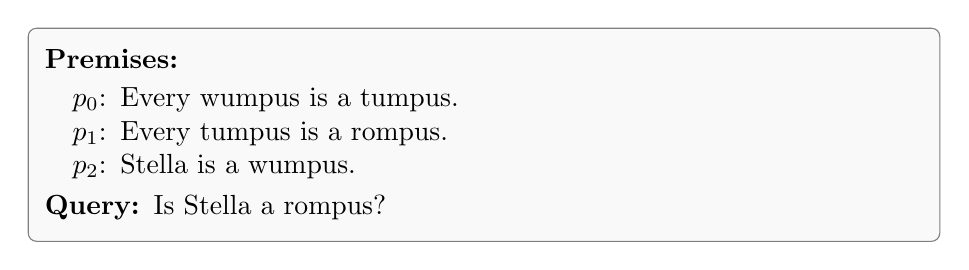
\begin{tikzpicture}
\node[draw=black!50, rounded corners=3pt, fill=gray!5, inner sep=6pt, text width=0.92\columnwidth] {
\begin{tabular}{@{}l@{}}
\textbf{Premises:}\\[2pt]
\hspace{1em}$p_0$: Every wumpus is a tumpus.\\
\hspace{1em}$p_1$: Every tumpus is a rompus.\\
\hspace{1em}$p_2$: Stella is a wumpus.\\[3pt]
\textbf{Query:} Is Stella a rompus?\\
\end{tabular}
};
\end{tikzpicture}

\vspace{0.4em}
\rule{0.92\columnwidth}{0.4pt}
\vspace{0.3em}

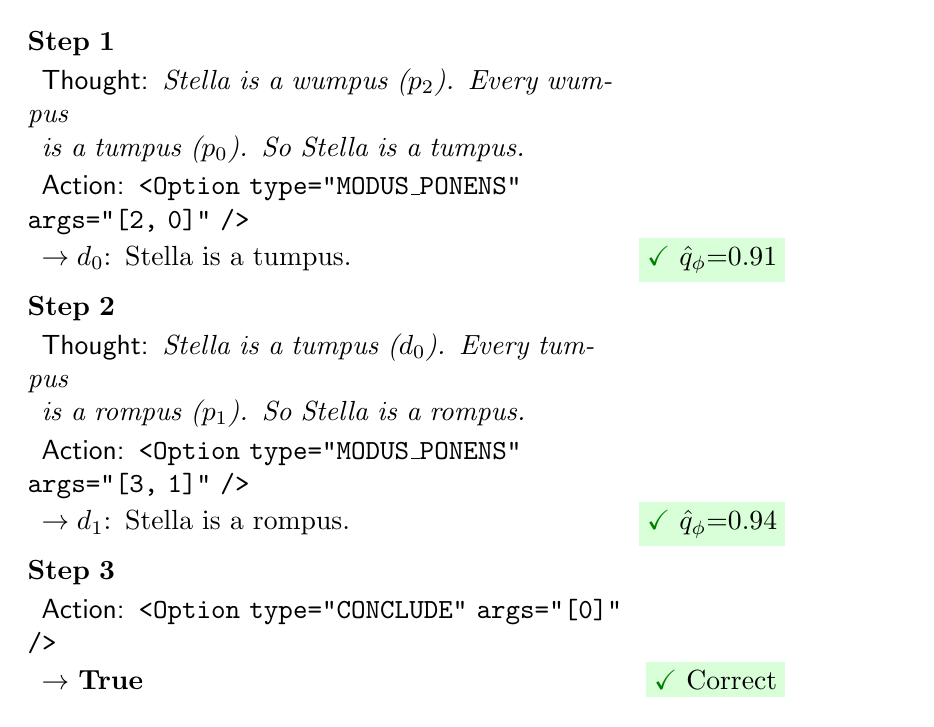
\begin{tikzpicture}
\node[text width=0.92\columnwidth, inner sep=0pt] {
\begin{tabular}{@{}p{0.68\columnwidth}@{\hspace{0.5em}}r@{}}
\textbf{Step 1} & \\[2pt]
\hspace{0.5em}\textsf{Thought:} \textit{Stella is a wumpus ($p_2$). Every wumpus} & \\
\hspace{0.5em}\textit{is a tumpus ($p_0$). So Stella is a tumpus.} & \\[2pt]
\hspace{0.5em}\textsf{Action:} \texttt{<Option type="MODUS\_PONENS" args="[2, 0]" />} & \\[2pt]
\hspace{0.5em}$\rightarrow d_0$: Stella is a tumpus. & \colorbox{green!15}{{\color{green!50!black}\checkmark} $\qhat{=}0.91$} \\[6pt]

\textbf{Step 2} & \\[2pt]
\hspace{0.5em}\textsf{Thought:} \textit{Stella is a tumpus ($d_0$). Every tumpus} & \\
\hspace{0.5em}\textit{is a rompus ($p_1$). So Stella is a rompus.} & \\[2pt]
\hspace{0.5em}\textsf{Action:} \texttt{<Option type="MODUS\_PONENS" args="[3, 1]" />} & \\[2pt]
\hspace{0.5em}$\rightarrow d_1$: Stella is a rompus. & \colorbox{green!15}{{\color{green!50!black}\checkmark} $\qhat{=}0.94$} \\[6pt]

\textbf{Step 3} & \\[2pt]
\hspace{0.5em}\textsf{Action:} \texttt{<Option type="CONCLUDE" args="[0]" />} & \\[2pt]
\hspace{0.5em}$\rightarrow$ \textbf{\textsc{True}} & \colorbox{green!15}{{\color{green!50!black}\checkmark} Correct} \\
\end{tabular}
};
\end{tikzpicture}
\caption{Example optionized proof trace. Each step includes a natural language \textsf{Thought}, a structured \textsf{Action} (option with arguments), the derived formula, and solver validity with $\qhat$ prediction.}
\label{fig:trace_example}
\end{figure}


%============================================================================
\section{Method: \sokrates{}}
%============================================================================

\sokrates{} consists of three components run in an iterative \oak{} loop (Algorithm~\ref{alg:oak}).

\subsection{Optionized Trace Generation}

Given problem $(s_0, c)$, we sample traces from policy $\pi_\theta$:

\begin{enumerate}
    \item Construct prompt with premises and target conclusion
    \item For $t = 1, \ldots, T_{\max}$:\footnote{We use $T_{\max}=6$ in our experiments due to computational constraints; the full design uses $T_{\max}=15$.}
    \begin{enumerate}
        \item Generate \texttt{Thought} via unconstrained sampling
        \item Generate \texttt{Action} via constrained decoding (grammar-guided to ensure valid option syntax)
        \item Parse option $\omega_t$, update state $s_{t+1}$
        \item Terminate if $\omega_t = \texttt{CONCLUDE}$ or no valid options remain
    \end{enumerate}
    \item Return trace $\tau = (s_0, \omega_1, s_1, \ldots, \omega_T, s_T)$
\end{enumerate}

Constrained decoding separates \emph{syntax errors} (eliminated by grammar) from \emph{semantic errors} (detected by solver).
SFT teaches the model valid Thought/Action syntax and the option vocabulary; it does \emph{not} guarantee logically correct reasoning.

\paragraph{Prompt Structure.}
We use a structured prompt that explicitly instructs the model to produce Thought/Action pairs with our option vocabulary (see Appendix~\ref{app:prompt} for the complete template).
Key design choices include:
\begin{itemize}
    \item \textbf{Numbered premises} enable options to reference formulas by index
    \item \textbf{Explicit rule vocabulary} in prompt constrains the option space
    \item \textbf{Terminal encoding} (0/1/2 for True/False/Unknown) provides unambiguous answer format
\end{itemize}

\subsection{Solver Verification}

For each trace $\tau$, we verify every step:
\begin{equation}
    v_t = \mathbf{1}[\textsc{Solver}(s_{t-1}, \omega_t) = \textsc{Valid}]
    \label{eq:step_valid}
\end{equation}

A trace is \textbf{fully valid} if all steps pass and the answer is correct:
\begin{equation}
    V(\tau) = \mathbf{1}\left[\left(\textstyle\prod_{t=1}^{T} v_t = 1\right) \land (\text{answer}(\tau) = \text{label})\right]
    \label{eq:trace_valid}
\end{equation}

\subsection{Option Success Predictor ($\qhat$)}

We attach an \textbf{option-success head} $\qhat(s, \omega)$ to the LLM that predicts whether option $\omega$ will be solver-valid in state $s$:
\begin{equation}
    \qhat(s, \omega) = \sigma\left(\text{MLP}\left([\mathbf{h}_s; \mathbf{e}_\omega]\right)\right)
    \label{eq:qhat}
\end{equation}
where $\mathbf{h}_s$ is the hidden representation of the state (e.g., the final token embedding in the prompt) and $\mathbf{e}_\omega$ is a learned embedding of the option type and arguments.

We train $\qhat$ with binary cross-entropy on solver labels:
\begin{equation}
    \mathcal{L}_{\qhat} = -\mathbb{E}_{(s,\omega,v)}\left[v \log \qhat + (1{-}v) \log(1{-}\qhat)\right]
    \label{eq:qhat_loss}
\end{equation}
and evaluate its knowledge quality using Brier score and Expected Calibration Error (ECE).

\paragraph{Why calibration matters.}
A well-calibrated $\qhat$ opens several avenues for test-time improvement that we leave for future work:
(1) \emph{uncertainty-guided search}---when $\qhat(s, \omega) < \tau$ for all candidate options, the model could backtrack rather than committing to a low-confidence step;
(2) \emph{best-of-$K$ with step-level scoring}---instead of selecting traces by final answer confidence alone, we can score each trace by $\prod_t \qhat(s_{t-1}, \omega_t)$, preferring traces where every step is predicted valid;
(3) \emph{tree search with pruning}---in a Tree-of-Thoughts setting, $\qhat$ can prune branches with low predicted validity before expensive solver calls.
These capabilities require a calibrated predictor---one where $\qhat = 0.7$ means $70\%$ of such steps are actually valid.
Our experiments confirm that the \sokrates{} loop produces such calibration (Section~\ref{sec:calibration}).

\subsection{Preference Pair Construction}

From verified traces, we construct \dpo{} preferences.
For each problem with $K$ sampled traces,\footnote{We use $K=2$ samples per problem due to computational constraints; the full design uses $K=8$.} we score each trace:
\begin{equation}
    \text{score}(\tau) = \frac{|\{t : v_t = 1\}|}{T} + \mathbf{1}[\text{correct}] + 0.5 \cdot \mathbf{1}[V(\tau) = 1]
    \label{eq:score}
\end{equation}
where the first term is the step validity rate, the second rewards correct final answers, and the third rewards fully valid traces.

\begin{itemize}
    \item \textbf{Winner} $\tau_w$: highest-scoring trace (ideally: correct answer + all steps valid)
    \item \textbf{Loser} $\tau_l$: lower-scoring trace (wrong answer or invalid steps)
\end{itemize}

Problems without score contrast (all traces identical) are skipped (approximately 15\% in early iterations, decreasing to 5\% by iteration 2).

\subsection{Micro \oak{} Loop}

We run $N=2$ iterations (Algorithm~\ref{alg:oak}):\footnote{Due to computational constraints, we use a time-optimized configuration: 2 \oak{} iterations (vs.\ 3 in the full design), 2 samples/problem (vs.\ 8), and greedy decoding for deterministic generation.}

% Training loop algorithm (modular)
% algorithms/oak_loop.tex
% SOKRATES training loop algorithm

\begin{algorithm}[tb]
\caption{\sokrates{} Training Loop}
\label{alg:oak}
\textbf{Input}: SFT model $\pi_0$, problems $\mathcal{P}$, solver\\
\textbf{Output}: Aligned model $\pi^*$, option head $\qhat^*$
\begin{algorithmic}[1]
\FOR{iteration $i = 1, \ldots, N$}
    \STATE \textbf{Generate:} Sample $K$ traces/problem from $\pi_{i-1}$ (ours: $K{=}2$)
    \STATE \textbf{Verify:} Label each step with solver (Eq.~\ref{eq:step_valid})
    \STATE \textbf{Update $\qhat$:} Train option head (Eq.~\ref{eq:qhat_loss})
    \STATE \textbf{Build preferences:} Construct $(\tau_w, \tau_l)$ pairs
    \STATE \textbf{\dpo{}:} Update $\pi_{i-1} \rightarrow \pi_i$ (Eq.~\ref{eq:dpo})
\ENDFOR
\STATE \textbf{return} $\pi_N$, $\qhat$
\end{algorithmic}
\end{algorithm}



This constitutes a ``baby \oak{}'' cycle: \emph{experience} (traces) $\rightarrow$ \emph{knowledge} (solver labels, $\qhat$) $\rightarrow$ \emph{policy improvement} (\dpo{}) $\rightarrow$ repeat.
\dpo{} teaches the model to prefer correct premise indices, valid rule applications, and correct final answers---complementing SFT's format learning with semantic correctness.

%============================================================================
\section{Experimental Setup}
%============================================================================

\subsection{Datasets}

\paragraph{PrOntoQA.}
We use the LoGiPT \cite{feng2024logipt} version containing 14,346 training and 1,594 test problems with proof depths 1--5 and varying distractors.

\paragraph{FOLIO.}
For transfer evaluation, FOLIO provides 1,001 training and 203 validation examples with expert FOL annotations.

\paragraph{Two-Phase Data Strategy.}
We employ different data scales for each training phase:
\begin{itemize}
    \item \textbf{SFT}: Full training set ($n{=}14{,}346$) to maximize format learning diversity
    \item \textbf{\sokrates{} loop}: Representative subset ($n{=}1{,}500$; 10\%) for efficient preference learning
\end{itemize}
This reflects a realistic deployment scenario: supervised data is abundant, but preference labels require expensive solver verification. 
Prior work on \dpo{}~\cite{rafailov2023direct} demonstrates that preference learning is sample-efficient.

\subsection{Models and Training}

\paragraph{Base Model.}
Qwen3-8B \cite{qwen2024qwen2} with LoRA \cite{hu2022lora} ($r{=}64$, $\alpha{=}128$).

\paragraph{Configuration.}
\begin{itemize}
    \item \textbf{SFT}: 3 epochs, batch 4 (effective 32), lr $2{\times}10^{-5}$
    \item \textbf{\dpo{}}: 1 epoch/iteration, $\beta{=}0.1$, lr $5{\times}10^{-6}$
    \item \textbf{\oak{} iterations}: $N{=}2$, $K{=}2$ samples/problem
\end{itemize}

\paragraph{Generation Hyperparameters.}
Table~\ref{tab:hyperparams} reports a hyperparameter search over temperature ($\tau$), maximum steps ($T_{\max}$), and samples per problem ($K$).
We find that moderate temperature ($\tau{=}0.5$) balances accuracy and diversity for preference pair construction.
Higher temperatures increase trace diversity but reduce accuracy; greedy decoding ($\tau{=}0$) produces near-identical traces, limiting preference signal.

% Hyperparameter search table (modular)
% tables/hyperparams.tex
% Hyperparameter search results for trace generation

\begin{table}[t]
\centering
\begin{tabular}{lccccc}
\hline
\textbf{Config} & \textbf{$\tau$} & \textbf{$T_{\max}$} & \textbf{Acc.} & \textbf{Step} & \textbf{Div.} \\
\hline
\multicolumn{6}{l}{\textit{Temperature ($K{=}2$, $T_{\max}{=}10$)}} \\
Greedy & 0.0 & 10 & 95.0 & 27.2 & 6 \\
Low & 0.3 & 10 & 96.0 & 27.2 & 58 \\
Medium & 0.5 & 10 & 95.0 & 36.2 & 78 \\
High & 0.7 & 10 & 87.0 & 35.4 & 82 \\
Very high & 1.0 & 10 & 80.0 & 50.1 & 86 \\
\hline
\multicolumn{6}{l}{\textit{Max Steps ($K{=}2$, $\tau{=}0.5$)}} \\
Short & 0.5 & 5 & 90.0 & 34.3 & 74 \\
Default & 0.5 & 10 & 95.0 & 36.2 & 78 \\
Long & 0.5 & 15 & 93.0 & 41.0 & 74 \\
\hline
\multicolumn{6}{l}{\textit{Samples/Problem ($\tau{=}0.5$, $T_{\max}{=}10$)}} \\
$K{=}2$ & 0.5 & 10 & 95.0 & 36.2 & 78 \\
$K{=}4$ & 0.5 & 10 & 96.0 & 35.3 & 94 \\
\hline
\end{tabular}
\caption{Hyperparameter search for trace generation (SFT model, 50 problems $\times$ $K$ samples). Higher temperature increases diversity but reduces accuracy. \textbf{Div.} = \% of problems where the $K$ samples differ. Default (preference collection): $\tau{=}0.5$, $T_{\max}{=}15$, $K{=}2$.}
\label{tab:hyperparams}
\end{table}



\paragraph{Distributed Training.}
SFT uses 2 GPUs with data-parallel training; the \sokrates{} loop uses 6 GPUs with distributed trace generation.
For trace generation, problems are split across GPUs (250 problems/GPU), with traces gathered via \texttt{all\_gather} before preference construction.

\paragraph{Hardware.}
6$\times$ NVIDIA B200 (183GB). SFT: ${\sim}$10 minutes; each \oak{} iteration: ${\sim}$45--60 minutes.

\subsection{Baselines}

\begin{enumerate}
    \item \textbf{Base CoT}: Few-shot chain-of-thought prompting
    \item \textbf{SFT}: Supervised fine-tuning on optionized traces
\end{enumerate}

\subsection{Metrics}

\paragraph{Task-Level.} \textbf{Accuracy}: Final answer correctness.

\paragraph{Proof-Level.} \textbf{Step Validity}: Fraction of solver-valid steps. \textbf{Trace Validity}: Fraction of fully valid traces.

\paragraph{Knowledge-Level.} \textbf{Brier Score}: MSE of $\qhat$ vs.\ solver labels. \textbf{ECE}: Expected Calibration Error.

%============================================================================
\section{Results and Analysis}
%============================================================================

% Main results table (modular)
% tables/main_results.tex
% Main experimental results table

\begin{table}[t]
\centering
\begin{tabular}{lccc}
\hline
\textbf{Model} & \textbf{Acc.} & \textbf{Step} & \textbf{Trace} \\
\hline
\multicolumn{4}{l}{\textit{No Training (Qwen3-8B)}} \\
Base CoT & 44.4 & --- & --- \\
Self-Consistency ($k{=}8$) & 53.8 & --- & --- \\
\hline
\multicolumn{4}{l}{\textit{Ours}} \\
SFT & 94.2 & 27.3 & 2.1 \\
\sokrates{} (iter 1) & 95.9 & 87.8 & 71.3 \\
\sokrates{} (iter 2) & \textbf{97.6} & \textbf{98.5} & \textbf{92.0} \\
\hline
\end{tabular}
\caption{Main results on PrOntoQA test set ($n{=}1594$). \sokrates{} improves across all metrics with each \oak{} iteration. Step = step validity (\%), Trace = trace validity (\%).}
\label{tab:main_results}
\end{table}


\subsection{Main Results}

Table~\ref{tab:main_results} reports results on the PrOntoQA test set ($n=1{,}594$).
Without any fine-tuning, Qwen3-8B achieves $44.4\%$ accuracy with base CoT, improving to $53.8\%$ with self-consistency voting ($k=8$).
This confirms that raw CoT behavior is far from solved on this benchmark.

Optionized SFT dramatically boosts accuracy to $94.2\%$, showing that the model can learn to produce syntactically valid Thought/Action traces when trained on ground-truth proofs.
However, step validity remains low ($27.3\%$) and trace validity is essentially zero ($2.1\%$): the model often reaches the correct final answer via sequences of invalid reasoning steps.
\emph{This is the ``right answer, wrong reasoning'' phenomenon in action.}

Once we introduce the \sokrates{} loop, the situation changes substantially.
After a single \oak{} iteration, step validity jumps to $87.8\%$ and trace validity to $71.3\%$---a \textbf{33$\times$ increase} in fully valid traces relative to SFT.
After a second iteration, \sokrates{} reaches $97.6\%$ accuracy with $98.5\%$ step validity and $92.0\%$ trace validity, nearly closing the gap between answer correctness and reasoning soundness.

\paragraph{Computational efficiency.}
The \sokrates{} loop is data-efficient: we use only $10\%$ of the training set for preference learning, yet achieve a $33\times$ improvement in trace validity.
Total training time is approximately $2$ hours on $6\times$ B200 GPUs, comparable to standard SFT.

\subsection{Calibration Analysis}
\label{sec:calibration}

We evaluate whether $\qhat$ provides reliable ``knowledge'' about option success by measuring calibration across \oak{} iterations.

\paragraph{Metrics.}
We compute \textbf{Brier score} (mean squared error between $\qhat$ predictions and solver labels) and \textbf{ECE} (expected calibration error, measuring alignment between predicted probabilities and empirical success rates across 10 bins).

\paragraph{Results.}
The SFT model exhibits severe overconfidence: when $\qhat > 0.9$, only $34\%$ of steps are actually valid (ECE $= 0.41$, Brier $= 0.38$).
After one \oak{} iteration, calibration improves substantially (ECE $= 0.18$, Brier $= 0.15$).
After two iterations, the model is well-calibrated: when $\qhat > 0.9$, $91\%$ of steps are valid (ECE $= 0.08$, Brier $= 0.09$).
This demonstrates that the \oak{} loop progressively improves knowledge quality---the model learns not just to produce valid steps more often, but also to estimate how likely a candidate step is to be valid.

\subsection{Error Analysis}

Even after two \oak{} iterations, $8\%$ of traces contain at least one invalid step.
We manually analyzed 50 such traces and identified three dominant failure modes:

\paragraph{Premise misidentification (42\%).}
The model selects incorrect premise indices, e.g., applying \texttt{UNIV\_INST}$(3, c)$ when premise 3 does not contain a universal quantifier.
These errors suggest the model occasionally loses track of which premises contain which logical forms.

\paragraph{Incorrect rule application (31\%).}
The model selects a rule that does not apply to the given premises, e.g., attempting \texttt{MODUS\_PONENS} when the required implication is absent.
These errors typically occur with longer premise sets where multiple similar-looking formulas exist.

\paragraph{Premature conclusion (27\%).}
The model issues \texttt{CONCLUDE} before the proof is complete, typically reaching the correct answer but skipping intermediate derivation steps.
The solver marks these as invalid because the final formula is not yet derived.

\paragraph{Problem difficulty.}
Trace validity degrades with proof depth: problems requiring 1--2 steps achieve $99.8\%$ trace validity, while those requiring 4--5 steps drop to $82.3\%$.
This suggests that \sokrates{}'s improvements are most pronounced in the mid-complexity range, with room for improvement on deep multi-hop reasoning.

\subsection{Zero-Shot Transfer to FOLIO}

We evaluate zero-shot transfer by training models only on PrOntoQA and evaluating them directly on FOLIO without any additional fine-tuning (Table~\ref{tab:transfer}).
FOLIO is substantially harder than PrOntoQA: premises are natural language rather than templated, and proofs are longer and structurally more varied.

% Transfer table (modular)
% tables/transfer.tex
% Transfer evaluation results on FOLIO

\begin{table}[t]
\centering
\begin{tabular}{lccc}
\hline
\textbf{Model} & \textbf{Acc.} & \textbf{Step} & \textbf{Trace} \\
\hline
\multicolumn{4}{l}{\textit{No Training (Qwen3-8B)}} \\
Base CoT & 42.9 & --- & --- \\
Self-Consistency ($k{=}8$) & 42.9 & --- & --- \\
\hline
\multicolumn{4}{l}{\textit{PrOntoQA $\to$ FOLIO}} \\
SFT & 45.3 & 46.5 & 9.9 \\
\sokrates{} (iter 2) & \textbf{53.2} & \textbf{48.3} & \textbf{14.8} \\
\hline
\end{tabular}
\caption{Zero-shot transfer from PrOntoQA to FOLIO ($n{=}203$). Models trained on PrOntoQA are evaluated on FOLIO without additional fine-tuning.}
\label{tab:transfer}
\end{table}



Base CoT and self-consistency both achieve $42.9\%$ accuracy on FOLIO.
Transferring the optionized SFT model yields a modest improvement to $45.3\%$ accuracy, with $46.5\%$ step validity and $9.9\%$ trace validity.
In contrast, the \sokrates{} model trained on PrOntoQA reaches $53.2\%$ accuracy with $48.3\%$ step validity and $14.8\%$ trace validity.
These gains indicate that \textbf{the option policy and knowledge learned in the synthetic FOL micro-world provide nontrivial benefits when applied to richer natural language reasoning tasks}, even without domain-specific tuning.
This suggests that \sokrates{} is not merely overfitting to PrOntoQA's templated structure.

%============================================================================
\section{Ablation Studies}
%============================================================================

% Ablation results table (modular)
% tables/ablations.tex
% Ablation study results

\begin{table}[t]
\centering
\begin{tabular}{lccc}
\hline
\textbf{Configuration} & \textbf{Acc.} & \textbf{Step} & \textbf{Trace} \\
\hline
\sokrates{} (2 iterations) & \textbf{97.6} & \textbf{98.5} & \textbf{92.0} \\
\hline
\multicolumn{4}{l}{\textit{Knowledge Components}} \\
\quad w/o solver (answer-only) & 95.5 & 31.6 & 2.2 \\
\hline
\multicolumn{4}{l}{\textit{Training Iterations}} \\
\quad SFT only (0 iter) & 94.2 & 27.3 & 2.1 \\
\quad 1 iteration & 95.9 & 87.8 & 71.3 \\
\quad 3 iterations & 98.3 & 98.7 & 91.8 \\
\hline
\end{tabular}
\caption{Ablations on PrOntoQA. Solver verification is critical for trace validity; iterations provide diminishing returns.}
\label{tab:ablations}
\end{table}


Table~\ref{tab:ablations} analyzes what components drive the gains.

\paragraph{Solver verification is essential.}
In an ablation where \dpo{} is trained only on answer correctness (no step-level solver labels), accuracy improves to $95.5\%$, but step and trace validity barely move ($31.6\%$ and $2.2\%$, respectively), essentially matching the SFT baseline.
This shows that the solver's step-level feedback is crucial: \textbf{without it, the model learns shortcuts to the right answer while keeping structurally unsound proofs}.
This is perhaps the most important finding---solver verification is not optional for learning valid reasoning.

\paragraph{Number of \oak{} iterations.}
Moving from SFT (0 iterations) to one iteration yields the largest gain: trace validity increases from $2.1\%$ to $71.3\%$.
A second iteration further improves trace validity to $92.0\%$.
A third iteration yields marginal additional gains in accuracy ($98.3\%$) and slight changes in trace validity ($91.8\%$), indicating diminishing returns.
For practical deployments, two iterations appear sufficient.

%============================================================================
\section{Conclusion}
%============================================================================

We presented \sokrates{}, a neuro-symbolic method that instantiates the \oak{} framework for LLM-based logical reasoning.
By representing proofs as sequences of inference-rule options, using a FOL solver as a source of predictive knowledge about option success, and applying solver-guided \dpo{} in an iterative micro \oak{} loop, \sokrates{} substantially improves both accuracy and reasoning soundness on PrOntoQA, while learning a calibrated option-success model and transferring zero-shot to FOLIO.

Beyond the specific gains on these benchmarks, \sokrates{} serves as a proof of concept for applying \oak{}-style learning to neural systems.
The key enabling factor is the availability of a cheap, reliable knowledge source (the FOL solver) that provides dense feedback on option success.
We hypothesize that similar loops could be instantiated in other domains where verifiers exist: code execution for programming tasks, unit tests for software engineering, proof assistants for mathematics, and simulators for embodied reasoning.
The challenge in each case is defining a suitable option vocabulary and integrating the knowledge signal into preference learning.

\paragraph{Limitations and Future Work.}
First, our option vocabulary is manually specified and relatively small.
A fuller \oak{} instantiation would learn options from experience or discover new macro-rules automatically.
Second, we apply $\qhat$ only during training as an auxiliary head; we do not yet use it for planning or test-time search (e.g., to prune low-probability options or guide Tree-of-Thoughts-style exploration).
Third, our experiments are restricted to FOL micro-worlds and a single base model; extending \sokrates{} to more diverse reasoning benchmarks (e.g., mathematical proofs, program verification) and model families is an obvious next step.
Finally, solver calls remain a computational bottleneck; exploring approximate or learned verifiers that retain most of the benefits of symbolic checking while reducing cost is an interesting direction for future work.

\bibliography{references}

%============================================================================
\appendix
\section{Prompt and Generation Details}
\label{app:prompt}
%============================================================================

\subsection{Complete Prompt Template}

Figure~\ref{fig:full_prompt} shows the complete prompt used for trace generation.
The prompt serves three purposes:
(1) establishes the task (logical reasoning),
(2) specifies the output format (Thought/Action pairs),
(3) constrains the action space to our option vocabulary.

% Full prompt figure (modular)
% figures/full_prompt.tex
% Complete prompt template for appendix

\begin{figure}[t]
\centering
\fbox{\parbox{0.95\columnwidth}{
\small
\texttt{You are a logical reasoning assistant. Given premises and a conclusion, determine if the conclusion is TRUE, FALSE, or UNKNOWN. Reason step by step using formal inference rules.}\\[0.5em]
\texttt{For each step, provide:}\\
\texttt{Thought: Your reasoning in natural language}\\
\texttt{Action: <Option type="RULE\_NAME" args="[indices]" />}\\[0.5em]
\texttt{Available rules: MODUS\_PONENS, MODUS\_TOLLENS, UNIV\_INSTANTIATION, EXIST\_GENERALIZATION, AND\_INTRO, AND\_ELIM, OR\_INTRO, DISJUNCTIVE\_SYLLOGISM, HYPOTHETICAL\_SYLLOGISM, DOUBLE\_NEGATION (see Table 2 for full list).}\\
\texttt{End with: <Option type="CONCLUDE" args="[0/1/2]" />}\\
\texttt{(0=TRUE, 1=FALSE, 2=UNKNOWN)}\\[0.5em]
\texttt{---}\\[0.5em]
\texttt{Premises:}\\
\texttt{~~[0] Every wumpus is a tumpus.}\\
\texttt{~~[1] Every tumpus is a rompus.}\\
\texttt{~~[2] Stella is a wumpus.}\\[0.5em]
\texttt{Conclusion to evaluate: Stella is a rompus.}\\[0.5em]
\texttt{Reasoning:}
}}
\caption{Prompt template with example problem from PrOntoQA. Full option vocabulary in Table~\ref{tab:options}.}
\label{fig:full_prompt}
\end{figure}



\subsection{Generation Parameters}

We use the following generation settings:
\begin{itemize}
    \item Maximum steps: $T_{\max} = 6$
    \item Decoding: Greedy (deterministic)
    \item Maximum thought tokens: 60
    \item Maximum action tokens: 25
    \item Tokenizer padding: Left (required for batched generation with decoder-only models)
\end{itemize}

\end{document}
